% FIXME Ao final, deixe descomentada a linha correspondente ao numero de paginas
% que a sua defesa possui.
\documentclass[12pt, letterpaper, twoside]{book}

%%%%%%%%%%%%%%%%%%%%%%%%%%%% Configuração: pacotes %%%%%%%%%%%%%%%%%%%%%%%%%%%%
\input{pacotes}  % Arquivo com os pacotes.

%%%%%%%%%%%%%%%%%%%%%%%%% Configuração: dados pessoais %%%%%%%%%%%%%%%%%%%%%%%%%
% FIXME Substituir 'Nome completo do aluno' pelo seu nome.
\newcommand{\autor}{Nome completo do aluno}
% FIXME Se for do sexo feminino, descomente a linha a seguir.
% \def\femaleAuthor{}

% FIXME Substituir 'Título da defesa' pelo título da defesa.
\newcommand{\titulo}{Título da defesa}
% FIXME Se estiver no programa de mestrado, descomente a linha a seguir.
% \def\mestrado{}
% FIXME Deixe descomente apenas a linha referente ao departamento.
% \def\matematica{}
\def\aplicada{}
% \def\estatistica{}

% FIXME Substituir 'Nome completo do orientador' pelo nome completo do seu
% orientador.
\newcommand{\orientador}{Nome completo do orientador}
% FIXME Se for orientado por uma mulher, descomente a linha a seguir.
% \def\femaleOrientador{}

% FIXME Substituir 'Nome completo do coorientador' pelo nome completo do seu
% coorientador. Caso não tenha coorientador, comente a linha a seguir.
\newcommand{\coorientador}{Nome completo do coorientador}
% FIXME Se for coorientado por uma mulher, descomente a linha a seguir.
% \def\femaleCoorientador{}

% FIXME Substituir 'Ano' pelo ano em que ocorreu sua defesa.
\newcommand{\ano}{Ano}

%%%%%%%%%%%%%%%%%%%%%%%%%%% Configuração: definições %%%%%%%%%%%%%%%%%%%%%%%%%%%
%%%%%%%%%%%%%%%%%%%%%%%%%% Configuração: frontmatter %%%%%%%%%%%%%%%%%%%%%%%%%%
\appto\frontmatter{\pagestyle{plain}}  % Adiciona o estilo plano de página.


%%%%%%%%%%%%%%%%%%%%%%%%%% Configurações: referências %%%%%%%%%%%%%%%%%%%%%%%%%%
\addbibresource{tese.bib}


%%%%%%%%%%%%%%%%%%%%%%%%%%%%% Configurações: links %%%%%%%%%%%%%%%%%%%%%%%%%%%%%
\hypersetup{
% TODO Por padrão os links, no pdf, para equações, figuras, referencias,
% tabelas, urls são identificados por uma caixa colorida em volta do link. Essa
% caixa colorida não eh impressa mas pode atrapalhar a leitura para alguns. Se
% desejar removê-las descomente a linha abaixo.
% hidelinks,
hypertexnames=false,
pdftitle={\titulo},  % Não modifique esta linha.
pdfauthor={\autor}  % Não modifique esta linha.
}


%%%%%%%%%%%%%%%%%%%%%%%%%% Configurações: numeração %%%%%%%%%%%%%%%%%%%%%%%%%%
\numberwithin{equation}{section}
\numberwithin{section}{chapter}


%%%%%%%%%%%%%%%%%%%%%%%%%%%% Configurações: amsthm %%%%%%%%%%%%%%%%%%%%%%%%%%%%
% Altera o estilo dos Teoremas, Conjecturas, ... e os possíveis valores
% são: plain, definition e remark.
% \theoremstyle{definition}
% Definição dos Teoremas, Conjecturas, ... e numeração dos mesmos
\newtheorem{thm}{Teorema}[section]
\newtheorem{con}[thm]{Conjectura}
\newtheorem{cor}[thm]{Corolário}
\newtheorem{dfn}[thm]{Definição}
\newtheorem{exm}[thm]{Exemplo}
\newtheorem{lem}[thm]{Lema}
\newtheorem{obs}[thm]{Observação}
\newtheorem{pps}[thm]{Proposição}


%%%%%%%%%%%%%%%%%%%%%%%%%%%%%% Configurações: códigos %%%%%%%%%%%%%%%%%%%%%%%% 
\lstset{
basicstyle=\ttfamily,
keywordstyle=\bfseries\color{green!40!black},
commentstyle=\color{gray},
stringstyle=\color{Maroon},
identifierstyle=\color{Blue},
numbers=left,
numberstyle=\tiny,
breaklines=false
}


%%%%%%%%%%%%%%%%%%%%%%%%%%%%% Configurações: anexo %%%%%%%%%%%%%%%%%%%%%%%%%%%
\newcommand{\annexname}{Anexo}
\makeatletter
\newcommand\annex{\par
\setcounter{chapter}{0}%
\setcounter{section}{0}%
\gdef\@chapapp{\annexname}%
\gdef\thechapter{\@Roman\c@chapter}}
\makeatother



% TODO Inserir configurações adicionais aqui.
  % Arquivo com algumas configurações.

%%%%%%%%%%%%%%%%%%%%%%%%%% Início do texto da defesa %%%%%%%%%%%%%%%%%%%%%%%%%%%
\begin{document}
% WARNING Todas as paginas deverão ser numeradas.
%
% As paginas iniciais são numeradas com algoritmos romanos em sua forma
% minuscula.
\frontmatter
%
\input{capa}  % Não edite esse arquivo.
\newpage\mbox{}\thispagestyle{plain}\newpage  % Pagina em branco.
%
% WARNING A folha de rosto precisa ser assinada pelos orientadores.
% WARNING Você deve escanear como preto-e-branco.
% FIXME Substitua arquivo folha-de-rosto.pdf por uma copia escaneada, comente
% esta linha e descomente a próxima.
\input{folha-de-rosto}
% \includepdf{folha-de-rosto.pdf}
%
% WARNING A ficha catalográfica deve estar no verso da folha de rosto.
% WARNING Você deve escanear como preto-e-branco.
% FIXME O arquivo ficha-catalografica.pdf deve ser sobrescrito com uma cópia
% do arquivo pdf que a biblioteca lhe enviar.
\includepdf{ficha-catalografica}
%
% WARNING A folha de aprovação deve ser assinada pelos membros da banca apos a
% defesa.
% WARNING Você deve escanear como preto-e-branco.
% FIXME Substitua o arquivo folha-de-aprovacao.pdf por uma copia escaneada.
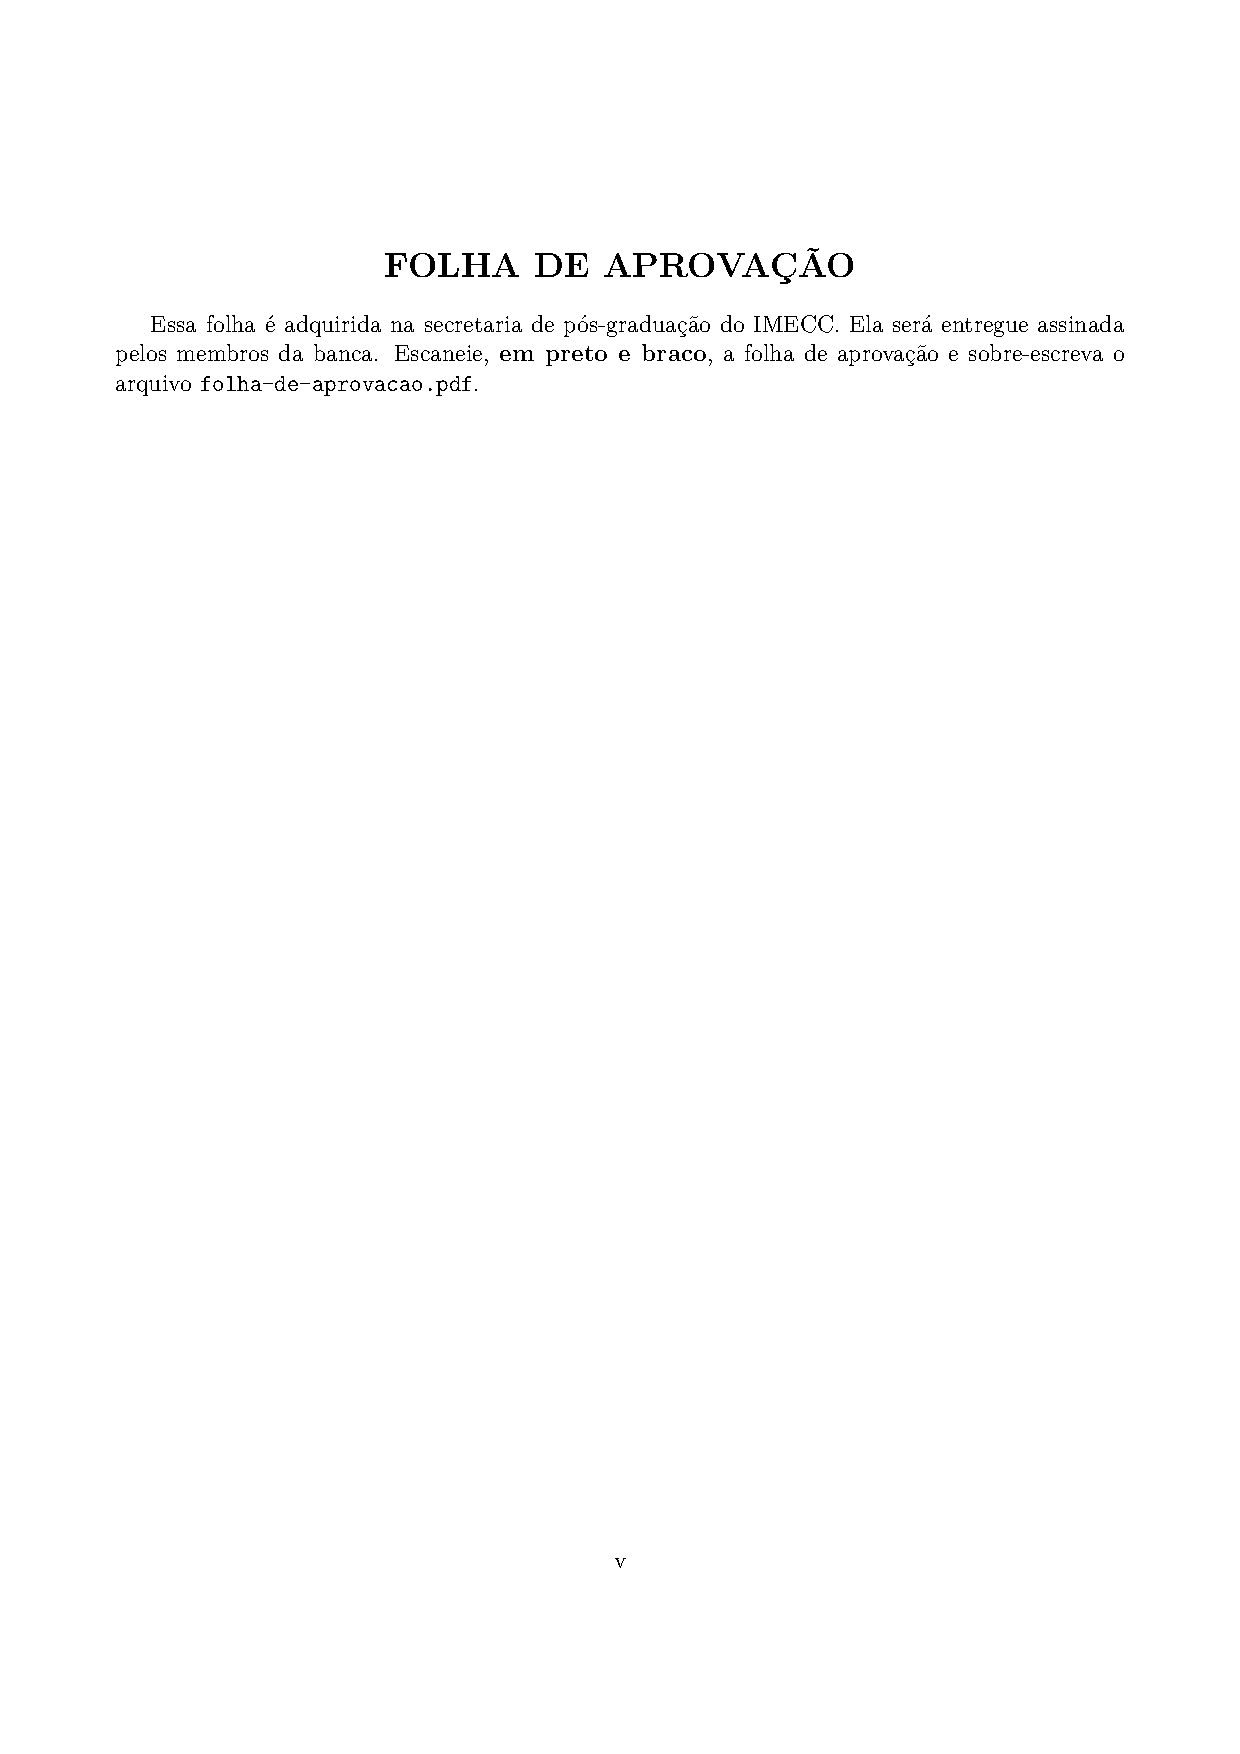
\includepdf{folha-de-aprovacao}
\chapter*{}  % Capítulo vazio.
\input{abstract}
\vspace{.1\textheight}
\input{resumo}
%
\tableofcontents
%
% FIXME Se não for incluir a dedicatória, comentar a linha abaixo.
\input{dedicatoria}
%
% FIXME Se não for incluir os agradecimentos, comentar a linha abaixo.
\input{agradecimentos}
%
% FIXME Comentar a linha abaixo se não desejar listar as figuras
% apresentadas.
\renewcommand{\listfigurename}{Lista de Ilustrações}  % CCPG 228/2013
\listoffigures
%
% FIXME Comentar a linha abaixo se não desejar listar as tabelas
% apresentadas.
\listoftables
%
% FIXME Comentar a linha abaixo de não for apresentar as
% abreviações e siglas utilizadas.
\input{abreviacoes}
%
% FIXME Comentar a linha abaixo se não for apresentar os
% símbolos utilizados.
\input{simbolos}
%
% FIXME Comentar a linha abaixo se não desejar listar os algoritmos
% apresentados.
\listofalgorithms
%
% FIXME Comentar a linha abaixo se não desejar listar os trechos de código
% apresentados.
\lstlistoflistings
%
% FIXME Ao final, se seu trabalho tiver menos de 100 páginas descomente as
% três linhas a seguir.
% \makeatletter
% \@openrightfalse
% \makeatother
%
% As paginas com o conteúdo da tese são numeradas com algoritmos arábicos.
\mainmatter
%
% FIXME Remover as 3 linhas abaixo.
\chapter{Título 1}
Esse é o primeiro capítulo da sua tese.

\section{Seção 1.1}
Essa é uma seção da sua tese.

\subsection{Subseção 1.1.1}

Essa é uma subseção da sua tese.

\subsection{Subseção 1.1.2}

Essa é outra subseção da sua tese.

\section{Equações matemáticas}
Para equações matemáticas está sendo utilizado os seguintes
pacotes:
\begin{itemize}
  \item amsmath,
  \item amsfonts,
  \item amssymb,
  \item amsthm,
  \item breqn.
\end{itemize}

Um exemplo de equação na mesma linha: 
$ 1 + 1 + 1 + 1 + 1 + 1 = 6$, 
que é trivial\index{trivial} de ser verificada.

Equações na mesma linha são quebradas automaticamente:
$ 1 + 1 + 1 + 1 + 1 + 1 + 1 + 1 + 1 + 1 + 1 + 1 = 12$. 

Ao utilizar equações na mesma linha deve-se tomar o cuidado de manter a
legibilidade da equação e não modificar a altura da linha. É
errado utilizar $\frac{1}{2} + \frac{1}{2} = 1$ ou $\frac{\partial}{\partial x}
(y^2 + 2xy + x^2) = 2y + 2x$, devendo ser utilizado $(1/2) + (1/2) = 1$ ou
$\partial (y^2 + 2 x y + x^2) / \partial x = 2 y + 2 x$.

Além de equações na mesma linha, também é possível
utilizar equações em destaque:
\begin{equation}
  1 + 1 + 1 + 1 + 1 + 1 = 6
\end{equation}
ou
\begin{equation*}
  1 + 1 + 1 + 1 + 1 + 1 = 6.
\end{equation*}
Ao utilizar equações matemáticas em destaque, não esqueça da pontuação nas
equações.

Recomenda-se utilizar os ambientes
\begin{itemize}
  \item dmath(*) e
  \item dgroup(*)
\end{itemize}
disponibilizados pelo pacote breqn ao invés dos ambientes
\begin{itemize}
  \item equation(*,)
  \item align(*),
  \item multiline(*) e
  \item split
\end{itemize}
pois os primeiros quebram e alinham automaticamente as equações em destaque.
Veja a seguir a ``equivalência'' entre os ambientes:
\begin{description}
  \item[dmath]
    \begin{dmath}
      1 + 1 + 1 + 1 + 1 + 1 + 1 + 1 + 1 + 1 + 1 + 1 + 1 + 1 + 1 + 1 + 1 + 1 + 1
      + 1 + 1 + 1 + 1 + 1 + 1 + 1 + 1 + 1 + 1 + 1 = 30
    \end{dmath}
  \item[equation] 
    \begin{equation}
      1 + 1 + 1 + 1 + 1 + 1 + 1 + 1 + 1 + 1 + 1 + 1 + 1 + 1 + 1 + 1 + 1 + 1 + 1
      + 1 + 1 + 1 + 1 + 1 + 1 + 1 + 1 + 1 + 1 + 1 = 30
    \end{equation}
  \item[equation com split] 
    \begin{equation}
      \begin{split}
        1 + 1 + 1 + 1 + 1 + 1 + 1 + 1 + 1 + 1 + 1 + 1 + 1 + 1 + 1 \\
        + 1 + 1 + 1 + 1 + 1 + 1 + 1 + 1 + 1 + 1 + 1 + 1 + 1 + 1 + 1 = 30 
      \end{split}
    \end{equation}
  \item[align] 
    \begin{align}
      1 + 1 + 1 + 1 + 1 + 1 + 1 + 1 + 1 + 1 + 1 + 1 + 1 + 1 + 1 \\
      + 1 + 1 + 1 + 1 + 1 + 1 + 1 + 1 + 1 + 1 + 1 + 1 + 1 + 1 + 1 = 30 
    \end{align}
  \item[align com quebra de linha] 
    \begin{align}
      1 + 1 + 1 + 1 + 1 + 1 + 1 + 1 + 1 + 1 + 1 + 1 + 1 + 1 + 1 \\
      + 1 + 1 + 1 + 1 + 1 + 1 + 1 + 1 + 1 + 1 + 1 + 1 + 1 + 1 + 1 = 30 
    \end{align}
\end{description}

No caso do desenvolvimento/simplificação de uma expressão
matemática também é recomendado utilizar os ambientes
disponibilizados pelo pacote breqn.
\begin{description}
  \item[dmath]
    \begin{dmath}
      f(x) = 1 + 1 + 1 + 1 + 1 + 1 + 1 + 1 + 1 + 1 + 1 + 1 + 1 + 1 + 1 + 1 + 1 +
      1 + 1 + 1 + 1 + 1 + 1 + 1 + 1 + 1 + 1 + 1 + 1 + 1
      = 2 + 2 + 2 + 2 + 2 + 2 + 2 + 2 + 2 + 2 + 2 + 2 + 2 + 2 + 2
      = 4 + 4 + 4 + 4 + 4 + 4 + 4 + 2
      = 8 + 8 + 8 + 6
      = 16 + 14
      = 30
    \end{dmath}
  \item[equation com split] 
    \begin{equation}
      \begin{split}
        f(x) &= 1 + 1 + 1 + 1 + 1 + 1 + 1 + 1 + 1 + 1 + 1 + 1 + 1 + 1 + 1 + 1 + 1 \\
        &\quad {}+ 1 + 1 + 1 + 1 + 1 + 1 + 1 + 1 + 1 + 1 + 1 + 1 + 1 \\
        &= 2 + 2 + 2 + 2 + 2 + 2 + 2 + 2 + 2 + 2 + 2 + 2 + 2 + 2 + 2 \\
        &= 4 + 4 + 4 + 4 + 4 + 4 + 4 + 2 \\
        &= 8 + 8 + 8 + 6 \\
        &= 16 + 14 \\
        &= 30
      \end{split}
    \end{equation}
  \item[align com quebra de linha] 
    \begin{align}
        f(x) &= 1 + 1 + 1 + 1 + 1 + 1 + 1 + 1 + 1 + 1 + 1 + 1 + 1 + 1 + 1 + 1 + 1 \\
        &\quad {}+ 1 + 1 + 1 + 1 + 1 + 1 + 1 + 1 + 1 + 1 + 1 + 1 + 1 \\
        &= 2 + 2 + 2 + 2 + 2 + 2 + 2 + 2 + 2 + 2 + 2 + 2 + 2 + 2 + 2 \\
        &= 4 + 4 + 4 + 4 + 4 + 4 + 4 + 2 \\
        &= 8 + 8 + 8 + 6 \\
        &= 16 + 14 \\
        &= 30
    \end{align}
\end{description}

Para o caso de equações relacionadas e que devem ser agrupadas,
temos
\begin{description}
  \item[dgroup com dmath]
    \begin{dgroup}
      \begin{dmath}
        f(x) = 1 + 1 + 1 + 1 + 1 + 1 + 1 + 1 + 1 + 1 + 1 + 1 + 1 + 1 + 1 + 1 + 1
        + 1 + 1 + 1 + 1 + 1 + 1 + 1 + 1 + 1 + 1 + 1 + 1 + 1
        = 2 + 2 + 2 + 2 + 2 + 2 + 2 + 2 + 2 + 2 + 2 + 2 + 2 + 2 + 2
        = 4 + 4 + 4 + 4 + 4 + 4 + 4 + 2
        = 8 + 8 + 8 + 6
        = 16 + 14
        = 30
      \end{dmath}
      \begin{dmath}
        g(x) = 2 + 2 + 2 + 2
        = 4 + 4
        = 8
      \end{dmath}
    \end{dgroup}
  \item[subequations com equation com split] 
    \begin{subequations}
      \begin{equation}
        \begin{split}
          f(x) &= 1 + 1 + 1 + 1 + 1 + 1 + 1 + 1 + 1 + 1 + 1 + 1 + 1 + 1 + 1 + 1 + 1 \\
          &\quad {}+ 1 + 1 + 1 + 1 + 1 + 1 + 1 + 1 + 1 + 1 + 1 + 1 + 1 \\
          &= 2 + 2 + 2 + 2 + 2 + 2 + 2 + 2 + 2 + 2 + 2 + 2 + 2 + 2 + 2 \\
          &= 4 + 4 + 4 + 4 + 4 + 4 + 4 + 2 \\
          &= 8 + 8 + 8 + 6 \\
          &= 16 + 14 \\
          &= 30
        \end{split}
      \end{equation}
      \begin{equation}
        \begin{split}
          g(x) &= 2 + 2 + 2 + 2 \\
          &= 4 + 4 \\
          &= 8
        \end{split}
      \end{equation}
    \end{subequations}
  \item[align com split] 
    \begin{align}
      \begin{split}
        f(x) &= 1 + 1 + 1 + 1 + 1 + 1 + 1 + 1 + 1 + 1 + 1 + 1 + 1 + 1 + 1 + 1 + 1 \\
        &\quad {}+ 1 + 1 + 1 + 1 + 1 + 1 + 1 + 1 + 1 + 1 + 1 + 1 + 1 \\
        &= 2 + 2 + 2 + 2 + 2 + 2 + 2 + 2 + 2 + 2 + 2 + 2 + 2 + 2 + 2 \\
        &= 4 + 4 + 4 + 4 + 4 + 4 + 4 + 2 \\
        &= 8 + 8 + 8 + 6 \\
        &= 16 + 14 \\
        &= 30
      \end{split} \\
      \begin{split}
        g(x) &= 2 + 2 + 2 + 2 \\
        &= 4 + 4 \\
        &= 8
      \end{split}
    \end{align}
\end{description}

\subsection{Referência cruzada}
Parte das equações anteriores encontram-se numeradas. Esse número pode ser
facilmente acessado se junto da equação tiver sido utilizando o comando label:
\begin{dmath}
  c^2 = a^2 + b^2. \label{eq:exem_pitagoras}
\end{dmath}
E para acessar o número utiliza o comando eqref, \eqref{eq:exem_pitagoras}.

Além de numerar equações também é possível nomeá-las utilizando o comando
tag\footnote{O pacote breqn não possue suporte ao comando tag.}:
\begin{align}
  c^2 &= a^2 + b^2 - 2 a b \cos\theta 
  \label{eq:exem_pitagoras_generalizado}
  \tag{GTP}
\end{align}
E para acessar o nome utiliza-se o comando eqref,
\eqref{eq:exem_pitagoras_generalizado}.

Para que no pdf não apareça o parâmetro dos comandos label é preciso remover o
pacote showlabels do arquivo pacotes.tex.

\section{Definições}
Vários ambientes já estão definidos como: Teorema, Conjectura, Corolário,
Definição, \ldots

\begin{thm}
  Teorema, Teorema, Teorema, Teorema.
\end{thm}
\begin{proof}
  Demostração do Teorema.
\end{proof}

\begin{con}
  Conjectura, Conjecture, Conjectura, Conjectura.
\end{con}
\begin{proof}
  Demostração do Conjectura.
\end{proof}

\begin{cor}
  Corolário, Corolário, Corolário, Corolário.
\end{cor}
\begin{proof}
  Demostração do Corolário.
\end{proof}

\begin{dfn}
  Definição, Definição, Definição.
\end{dfn}
\begin{proof}
  Demostração da Definição.
\end{proof}

Use esses ambientes de maneira sábia.

\input{ex_cap2}
\input{ex_cap3}
\input{ex_cap4}
%
% TODO Inserir os arquivos referentes ao corpo da tese.
%
% Referência bibliográfica.
\newpage
\phantomsection
\addcontentsline{toc}{chapter}{Referências}
\printbibliography[title=Referências]
%
% FIXME Se não for utilizar apêndices (o glossario é um apêndice), comentar a
% linha abaixo.
\appendix
% FIXME Remover as 4 linha abaixo.
\input{glossario}
\input{ex_ape1}
\input{ex_ape2}
\input{ex_ape3}
\input{ex_ape4}
% TODO Inserir os arquivos referentes aos apêndices.
%
% TODO Se não for utilizar anexos nem uma licença Creative Commons, comentar a linha abaixo.
\annex
% FIXME Remover a linha abaixo.
\input{ex_ane1}
% TODO Inserir os arquivos referentes aos anexos.
%
% FIXME Escolher, opcionalmente, uma das licença Creative Commons abaixo.
% Para isso remova a linha correspondente a licença não desejada.
\input{cc-by}  % Creative Commons Atribuição 3.0 Não Adaptada
\input{cc-by-sa}  % Creative Commons AtribuiçãoCompartilhaIgual 3.0 Não Adaptada
%
\clearpage
\backmatter
\phantomsection
\addcontentsline{toc}{chapter}{Índice Remissivo}
\printindex
\end{document}
